\lez{19}{01-04-2020}{Dagli appunti di Sara}
\subsection{Scattering elastico}
\label{subsec:Diffusione elasica}
Possiamo considerare lo scattering elastico come l'interazione di una sonda radiativa con la materia senza scambio di energia\footnote{Ovviamente il momento della sonda può invece cambiare}. Fissiamo le idee con la seguente Figura:
\begin{figure}[H]
    \centering
    \incfig{scattering-elastico-di-un-onda-elettromagnetica-con-un-blocco-di-materia}
    \caption{Scattering elastico di un onda elettromagnetica con un blocco di materia}
    \label{fig:scattering-elastico-di-un-onda-elettromagnetica-con-un-blocco-di-materia}
\end{figure}
\noindent
Dal valore di $\Delta\v{k}$ possiamo derivare molte proprietà del materiale disegnato come una sfera opaca in Figura \ref{fig:scattering-elastico-di-un-onda-elettromagnetica-con-un-blocco-di-materia}.\\
Abbiamo parlato di sonda radiativa, quindi di radiazione elettromagnetica. Per questo tipo di sonda abbiamo la relazione:
\[
	E_{\gamma} = E_\text{sonda}[\text{eV}] \sim \frac{1240}{\lambda [\text{nm}]}
.\] 
Vediamo quali tipi di sonde potrebbero esserci utili per studiare la struttura del nostro blocco di materiale (in particolare quali sonde sono adatte a fare scattering elastico):
\begin{description}
	\item[Microonde? No.] 
		Le microonde hanno energie molto basse, le loro frequenze sono risonanti con le vibrazioni reticolari corrispondenti ai fononi a bassa energia. 
		La radiazione sonda viene assorbita dal materiale sotto forma di assorbimento infrarosso.
	\item[Visibile? No.]
		Abbiamo energie dell'ordine dell'eV, queste energie sono solitamente risonanti con i salti tra i livelli elettronici.
		Gli elettroni possono assorbire questa radiazione e come conseguenza il materiale si potrebbe anche ionizzare. 
	\item[Raggi X? Si.]
		Questa radiazione ha energie superiori ai KeV con una lunghezza d'onda dello stesso ordine di grandezza della spaziatura tra gli atomi (1-10 \AA ). 
		Nella vasta regione dei raggi X si può avere ionizzazione degli atomi, scattering fotone-elettrone (Compton) ed in una regione intermedia di questa radiazione 
		anche scattering elastico (Thompson e Rayleigh). Questa ultima prevale in genere sulle altre due, questo rende la radiazione ai raggi X decente per questa analisi.\\
		Tuttavia questa sonda può sempre interagire con la materia carica, quindi oltre a sondare la posizione degli atomi si rileva anche la nube elettronica che li circonda,
		questo può essere un effetto negativo o positivo a seconda del motivo dello studio.
	\item[Neutroni? Si.]
		Non risentendo della interazione elettromagnetica i neutroni possono fare scattering elastico direttamente con i nuclei permettendo di vedere molto bene la struttura 
		del materiale sondato. Il problema dell'utilizzo di neutroni è la difficoltà nel produrre e gestire fasci di queste particelle.
	\item[Elettroni? No.] 
		Gli elettroni presentano sia le difficoltà dei Raggi X (poichè interagiscono) sia quelle dei neutroni (è difficile produrre fasci), sono quindi sfavorite per questo scopo.
\end{description}
\subsection{Fattore di struttura statistica.}
\label{subsec:Fattore di struttura statistica.}

Andiamo nel dettaglio della analisi incidendo con un'onda su un materiale ed inserendo un rilevatore dietro a quest'ultimo:
\begin{figure}[H]
    \centering
    \incfig{scattering-con-rilevatore}
    \caption{\scriptsize Scattering con rilevatore, a destra un pattern di rifrazione frutto di interferenza con le onde scatterate da centri scatteranti diversi.}
    \label{fig:scattering-con-rilevatore}
\end{figure}
\noindent
La risoluzione di questo tipo di tecniche dipende dal limite di diffrazione, quindi dal $\lambda$ della sonda. Tale $\lambda$ dovrà essere dello stesso ordine della distanza interatomica per poter vedere qualcosa.\\
Abbiamo un campo EM incidente la cui intensità è proporzionale al modulo quadro dell'ampiezza:
\[
	E_i = \phi_{i,0}(\v{r}) \sim e^{i \v{k}\v{r}} \implies I_0 \sim \left| \phi_{i,0} \right| ^2
.\] 
Gli atomi investiti da tale radiazione elettromagnetica si comportano come dipoli oscillanti (considerando il nucleo pesante e fermo), quindi riemettono in tutte le direzioni \footnote{In realtà le direzioni di emissione sono limitate per la radiazione di dipolo come ben sappiamo, tuttavia se ci restringiamo all'osservazione di una piccola zona possiamo assumere emissione uniforme} con gli stessi $\omega $ e $\lambda$.\\
Visto che i dipoli sono investiti con fasi differenti possiamo scrivere il campo emesso in prima approssimazione come:
\[\begin{aligned}
	\phi(r) \sim &
	\sum_{i}^{} 
	\underbrace{
	\phi_0 
	}_{\substack{\text{fase}\\ \text{iniziale}}}
	\underbrace{
	\frac{1}{\left| \v{r}-\v{r}_i \right|}
	\exp\left( i \v{k}\left( \v{r}-\v{r}_i \right) \right) 
	}_{\substack{\text{Campo}\\ \text{di particella}\\ \text{i-esima}}} \sim\\ 
	\sim &
	\exp\left( i \v{k}'\v{r}' \right) \sum_{i}^{} \exp\left( i \left( \v{k}-\v{k}' \right) \v{r}_i \right) 
.\end{aligned}\]
Facendo quindi il modulo quadro di questa espressione abbiamo l'intensità di scattering \footnote{Ogni media tra parentesi $\left< \right>$ è da intendersi come media statistica}:
\[
	I \sim I_0 \left< \left| \sum_{i}^{} \exp \left[ - i \v{q}\left( \v{r}_i - \v{r}_j \right)  \right]  \right|^2  \right>
.\] 
In quest'ultima è evidente che vi può essere interferenza tra i termini oscillanti all'interno della sommatoria, tale interferenza è quella che ci permette di avere informazioni sulla struttura interna. Normalizzando $I$ sulla intensità $I_0$ si ha:
\[
	\frac{I(\Delta\v{k})}{I_0} 
	=
	\frac{I(\v{k},\theta,\varphi)}{I_0}
	=
	\left< \sum_{i,j}^{} \exp\left( -i \Delta\v{k}\left( \v{r}_i - \v{r}_j \right)  \right)  \right>
.\] 
Dove abbiamo riscritto il modulo quadro tramite una doppia sommatoria.\\
Nel caso di scattering in avanti ($\Delta\v{k}=0$) possiamo dire che $I/I_0 = N^2$. Questo termine è sempre presente e non da informazioni sulla struttura interna, di conseguenza viene spesso oscurato (nella analisi matematica si rimuove con una $\delta$):
\[
	\frac{I(\Delta\v{k})}{I_0}-N^2\delta_{\v{k},\v{k}'}
.\] 
Vorremmo trattare il termine con $\Delta\v{k}=0$ come un termine incoerente, tuttavia questo scala come $N^2$ mentre i termini incoerenti scalano solitamente come $N$. Normalizzando il tutto otteniamo un importante parametro nella nostra analisi.
\begin{defn}[Fattore di struttura statistica]{def:Fattore di struttura statistica}
	Si definisce Fattore di struttura statistica la quantità: 
	\[\begin{aligned}
		S(\v{q}) 
		=&
		\frac{I(\v{q})}{N} - N \delta_{\v{q},0} 
		=\\=&
		\frac{1}{N}\left< \sum_{i,j}^{} \exp\left( -i \v{q}\left( \v{r}_i-\v{r}_j \right) \right) \right> - N\delta_{\v{q},0}
	.\end{aligned}\]
	In cui $\v{q}=\Delta\v{k}$.
\end{defn}
Notiamo che questa quantità gode di alcune proprietà interessanti:
\begin{itemize}
	\item Se $\v{q}=0$ allora $S(\v{q})=0$ ma $S(\v{q}\to 0) = \text{cost}$.
	\item Se $q\to \infty$ i termini esponenziali per $i\neq j$ oscillano molto rapidamente mediando a zero, prevalgono quindi i termini in diagonale, per questo 
		$S(\v{q}\to \infty)=1$.
\end{itemize}
Notiamo che se il sistema è composto da atomi di specie diverse ognuna di queste potrebbe avere intensità di scattering differente, quindi la sommatoria per $S(\v{q})$ dovrà essere pesata con i fattori di forma atomici.
\subsection{Densità ad uno e a due particelle.}
\label{subsec:Densità ad uno e a due particelle.}
Possiamo definire alcune quantità utili per l'analisi del fattore di struttura statistica: 
\begin{defn}[Densità ad una particella]{def:Densità ad una particella}
	Possiamo definire la densità di probabilità per una particella come:
	\[
		\rho (\v{r}) = \left<\sum_{i}^{} \delta\left( \v{r}_i - \v{r} \right)\right>
	.\] 
	Dove questa funzione ha la proprietà:
	\[
		\int\rho (\v{r})d \v{r} = N 
	.\] 
\end{defn}
Notiamo che questa è una quantità molto generale, la si usa in fisica 2 quando si dimostrano i potenziali di Lienard Wiechert (con Pegoraro) e la si applica anche in altre dimostrazioni.
\newpage
\begin{defn}[Densità di massa a due particelle]{def:Densità di massa a due particelle}
	La densità di massa a due particelle è definita come la probabilità che una particella sia in $\v{r}$ ed una in $\v{r}'$:
	\[\begin{aligned}
		\rho _2(\v{r},\v{r}') 
		=&
		\left<\sum_{i,j}^{} \delta\left( \v{r}_i-\v{r} \right) \delta\left( \v{r}_j-\v{r}' \right)  \right> =\\
		=&
		\left<\sum_{i\neq j}^{} \delta\left( \v{r}_i -\v{r} \right) \delta\left( \v{r}_j-\v{r}' \right)  \right>
		+
		\left<\sum_{i}^{} \delta\left( \v{r}_i-\v{r} \right) \delta\left( \v{r}_i -\v{r}' \right)  \right> = \\
		=&
		\overline{\rho}(\v{r},\v{r}') 
		+
		\left<\sum_{i}^{} \delta\left( \v{r}_i-\v{r} \right)\delta\left( \v{r}_i-\v{r}' \right)   \right>
	.\end{aligned}\]
\end{defn}
Notiamo quindi che vi è una duplice definizione, una che tiene conto della probabilità di trovare le due particelle nello stesso punto: $\rho _2$ ed una che invece rimuove questo termine poco fisico: $\overline{\rho }_2$.\\
La prima definizione ha una utilità puramente matematica, la seconda invece è accettabile fisicamente in ogni caso. Da notare che, nel limite termodinamico $N\to \infty$ le due quantità coincidono. Infine abbiamo che:
\[\begin{aligned}
	&\int\rho _2(\v{r},\v{r}')d \v{r}d \v{r}' = N^2\\
	&\int \overline{\rho } _2(\v{r},\v{r}')d \v{r}d \v{r}' = N^2 -N
.\end{aligned}\]
\subsection{Fattore di struttura statistica come trasformata di Fourier della densità a due particelle.}
\label{subsec:Fattore di struttura statistica come trasformata di Fourier della densità a due particelle.}
\subsubsection{Trasformata della densità ad una particella.}
\label{subsubsec:Trasformata della densità ad una particella.}
Effettuiamo prima questa trasformata:
\[\begin{aligned}
	FT(\rho (\v{r})) =&
	\int e^{i \v{k}\v{r}}\rho (\v{r})d \v{r} =\\
	=&
	\left<\sum_{i}^{} e^{i \v{k}\v{r}} \delta(\v{r}_i -\v{r})d \v{r} \right> =\\
	=&
	\left<\sum_{i}^{} e^{i \v{k}\v{r}_i} \right>
.\end{aligned}\]
Otteniamo una sommatoria su onde con fasi differenti.
\subsubsection{Trasformata della densità a due particelle.}
\label{subsubsec:Trasformata della densità a due particelle.}
Vogliamo calcolare la densità a due particelle che distano da una origine rispettivamente $\v{r}_1$ e $\v{r}_2$. Per effettuare il calcolo facciamo il seguente cambio di variabili:
\[\begin{aligned}
	&\v{r} = \v{r}_1-\v{r}_2 &&&&&&
	&\v{R} = \frac{\v{r}_1 + \v{r}_2}{2}
.\end{aligned}\]
In questo modo abbiamo che:
\[\begin{aligned}
	\rho (\v{r}_1,\v{r}_2) 
	=&
	\left<\sum_{i,j}^{} \delta(\v{r}_i - \v{r}_1)\delta(\v{r}_j - \v{r}_2) \right> =\\
	=&
	\left<\sum_{i,j}^{} \delta(\v{r}_i - \left( R + \frac{\v{r}}{2} \right) )\delta(\v{r}_j - \left( R - \frac{\v{r}}{2} \right)) \right> 
.\end{aligned}\]
Gli argomenti delle due $\delta$ si annullano quando
\[\begin{aligned}
	& \v{r}_i = \v{R}+\frac{\v{r}}{2}\\
	&\v{r}_j = \v{R}- \frac{\v{r}}{2}
.\end{aligned}\]
Sommando e sottraendo queste due equazioni possiamo riscrivere in maniera equivalente l'equazione per $\rho (\v{r}_1,\v{r}_2)$:
\[\begin{aligned}
	\rho (\v{r}_1, \v{r}_2) = &
	\rho (\v{r},\v{R}) =\\
	=&
	\left< \sum_{i,j}^{} \delta(\v{r}-\left( \v{r}_i-\v{r}_j \right))\delta\left(  \v{R}- \frac{\left( \v{r}_i + \v{r}_j \right) }{2} \right)  \right>
.\end{aligned}\]
Adesso facciamo una trasformata di Fourier rispetto ad $\v{R}$ e $\v{r}$:
\[\begin{aligned}
	FT(\rho_2 (\v{r}_1,\v{r}_2)) =&
	\left<\sum_{i,j}^{} \int \delta(\v{r} - \left( \v{r}_i -\v{r}_j \right) )e^{-i \v{q}\v{r}}d \v{r} 
	\int \delta \left( \v{R} - \frac{\left( \v{r}_i +\v{r}_j \right)}{2}  \right) e^{-i \v{Q}\v{R}}d \v{R} \right> =\\
	=&
	\left<\sum_{i,j}^{} 
	\underbrace{
	e^{-i \v{q}\left( \v{r}_i - \v{r}_j \right) } 
	}_{\sim S(\v{q})}
	\underbrace{
	e^{-i \v{Q}\left( \v{r}_i + \v{r}_j \right)/2 }
	}_{\sim FT(\rho (\v{r}))}
	\right>=\\
	=& \hat{S}(\v{q},\v{Q})
.\end{aligned}\]
Abbiamo quindi una importante relazione esatta che lega la densità a due al fattore di struttura statistica
\begin{fact}[Fattore di struttura statistica e densità a due legati da FT]{fact:Fattore di struttura statistica e densità a due legati da FT}
	Il fattore di struttura statistica può essere espresso come:
	\[\begin{aligned}
		S(\v{q}) 
		=&
		\frac{\hat{S}(\v{q},\v{Q}=0)}{N} - N \delta_{\v{q},\v{Q}=0} =\\
		=&
		\frac{1}{N}\int\int d \v{r}_1 d \v{r}_2e^{-i \v{q} \left( \v{\v{r}_1 - \v{r}_2} \right) }\rho _2 \left( \v{r}_1,\v{r}_2 \right) - N \delta_{\v{q},0}=\\
		=&
		\frac{1}{N}\int\int d \v{r} d \v{R}e^{-i \v{q}\v{r}}\rho _2 \left( \v{R} + \frac{\v{r}}{2}, \v{R}- \frac{\v{r}}{2} \right) - N \delta_{\v{q},0}
	.\end{aligned}\]
\end{fact}
\subsection{Fattore di struttura statistica per i liquidi}
\label{subsec:Fattore di struttura statistica per i liquidi}
Nel caso di un liquido uniforme ed isotropo abbiamo che 
\[
	\rho (\v{r}) = \rho = \frac{N}{V}
.\] 
Di conseguenza si ha che $\rho _2$ dipenderà soltanto dalla distanza $r = \left| \v{r}_1 - \v{r}_2 \right| $ e potrà essere scritto come:
\[
	\rho _2 (\v{r}_1, \v{r}_2) 
	=
	\rho ^2\left[ g(r)+V\delta(r) \right] 
.\] 
Dove la $g(r)$ è detta funzione di correlazione di coppia e tiene di conto del contributo a $\rho _2$ di particelle distinte mentre $V\delta(r)$ tiene di conto del contributo "self".\\
Notiamo anche che la funzione di correlazione di coppia è la funzione che ci permette di calcolare anche il numero di particelle nella shell sferica a distanza $r$ da una particella data:
\begin{figure}[H]
	\centering
	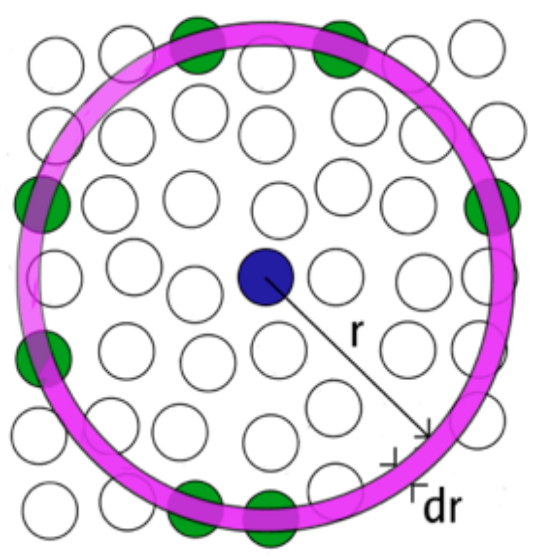
\includegraphics[width=0.2\textwidth]{figures/Istantanea_2020-04-04_09-36-23.png}
	\caption{Numero di particelle nella shell di raggio $r$.}
	\label{fig:-figures-Istantanea_2020-04-04_09-36-23-png}
\end{figure}
\[
	dN = \rho 4\pi r^2 g(r)dr
.\] 
Per questi sistemi possiamo scrivere il fattore di struttura statistica come:
\[\begin{aligned}
	S(q) =&
	\frac{\rho }{V} \int \left[ g(r) + V\delta(\v{r}) \right] e^{-i \v{q}\v{r}}d \v{r} - N \delta_{\v{q},0}=\\
	=&
	\frac{\rho }{V} \int \left[ g(r) + V\delta(\v{r}) \right] e^{-i \v{q}\v{r}}d \v{r} - \frac{N}{V^2} \int e^{-i \v{q}\v{r}}d \v{r}=\\
	=&
	1 + \rho \int_{0}^{\infty} \left[ g(r) - 1 \right] \frac{\sin(qr)}{qr}4\pi r^2 dr 
.\end{aligned}\]
\begin{fact}[Fattore di struttura statistica per i liquidi]{fact:Fttore di struttura statistica per i liquidi}
	\[
		S(q) - 1 = 
		\rho \int_{0}^{\infty} \left[ g(r) - 1 \right] \frac{\sin(qr)}{qr}4\pi r^2 dr 
		=
		FT\left[ g(r) - 1 \right] 
	.\] 
\end{fact}
Quindi vi è un evidente collegamento tra la trasformata di Fourier della $g(r)$ ed il fattore di struttura statistica.
\subsection{Fattore di struttura statistica per sistemi amorfi e cristallini}
\label{subsec:Fattore di struttura statistica per sistemi amorfi e cristallini}
I sistemi amorfi dal punto di vista dello scattering assomigliano molto ai liquidi, soltanto che la forma della $S(q)$ è molto più rumorosa che in questi ultimi.\\
Questo perché la media termodinamica è più efficiente nei liquidi (essendo le particelle in movimento con $v_\text{liq} \gg v_\text{amorfo} $).\\
Nei cristalli invece si ha che la densità può essere espressa come sovrapposizione di funzioni periodiche e localizzate nei siti in cui sono presenti gli atomi $\v{R}_I$:
\[
	\rho (\v{r}) 
	=
	\sum_{I}^{} f(\v{r}-\v{R}_I)
.\] 
La densità a due particelle invece è:
\[
	\overline{\rho} _2(\v{r}_1,\v{r}_2) 
	=
	\rho (\v{r}_1)\rho (\v{r}_2) - \delta(\v{r}_1-\v{r}_2)\rho (\v{r}_1)
.\] 
Contrariamente a quanto si ha per i liquidi la correlazione tra due siti differenti è molto bassa (gli atomi si muovono attorno a posizioni ben precise ma non si spostano molto lontano).\\
Possiamo esprimere quindi il fattore di struttura statistica come:
\[
	S(\v{q}) =
	1 + \frac{1}{N}\int \rho (\v{r}')\rho (\v{r}) e^{i \v{q}\left( \v{r}-\v{r}' \right) }d \v{r}d \v{r}'
	-
	\frac{1}{N}\int\delta(\v{r}-\v{r}')\rho (\v{r})e^{i \v{q}\left( \v{r}-\v{r}' \right)} d \v{r} d \v{r}' 
	- N \delta_{0,\v{q}}
.\] 
Quindi raggruppando qualche termine si ha:
\begin{fact}[Fattore di struttura statistica per i cristalli]{fact:Fattore di struttura statistica per i cristalli}
	\[
		S(\v{q}) + N \delta_{0,\v{q}} 
		=
		\frac{1}{N}\left| \int\rho (\v{r})e^{i \v{q}\v{r}} d \v{r} \right|^2 = \left| FT\left[ \rho (\v{r}) \right]  \right| ^2
	.\] 
\end{fact}
Quindi i punti visualizzati sul rilevatore sono espressione diretta della trasformata di $\rho (\v{r})$. \\
\subsection{Digressione sulla FT}
\label{subsec:Digressione sulla FT}
Posso descrivere un cristallo come una somma di funzioni centrate sui siti cristallini. In prima approssimazione supponiamo che tali funzioni siano delle $\delta$:
\[
	\rho (\v{r}) = \sum_{I}^{} f(\v{r}-\v{R}_I) = \sum_{I}^{} \delta(\v{r}-\v{R}_I)
.\] 
La trasformata di Fourier di una tale funzione sarà:
\[\begin{aligned}
	FT\left[ \rho (\v{r}) \right] 
	=&
	\frac{1}{V}\int \sum_{I}^{} \delta(\v{r}-\v{R}_I)e^{i \v{q}\v{r}}d \v{r} =\\
	=&
	\frac{1}{V}\sum_{I}^{} e^{i \v{q}\v{R}_I} =\\
	=&
	\frac{N}{V}\sum_{J}^{} \delta_{\v{k},\v{K}_J}
.\end{aligned}\]
Quindi una periodicità in spazio reale corrisponde ad una discretizzazione dello spazio reciproco. \\
Quest'ultima affermazione equivale a dire che il rapporto tra reticolo diretto e reciproco è l'equivalente della condizione di Bragg di interferenza costruttiva ($e^{-i \v{R}\v{K}} = 1$).
\begin{figure}[H]
	\centering
	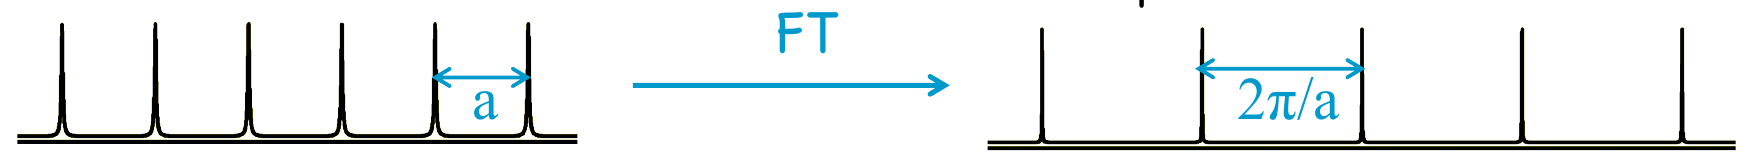
\includegraphics[width=0.6\textwidth]{figures/reticolo-localizzato.png}
	\caption{trasformata della $\rho (r)$ nel caso di reticolo perfettamente localizzato.}
	\label{fig:}
\end{figure}
\noindent
In realtà gli elettroni formano una nube delocalizzata attorno agli atomi della struttura, quindi per usare una $\rho (\v{r})$ più realistica dovremmo prendere dei picchi gaussiani anziché le $\delta$. Facendo in questo modo nel reticolo reciproco rimangono delle $\delta$ di Kronecker ma i picchi di quest'ultime non saranno ad altezza costante:
\begin{figure}[H]
	\centering
	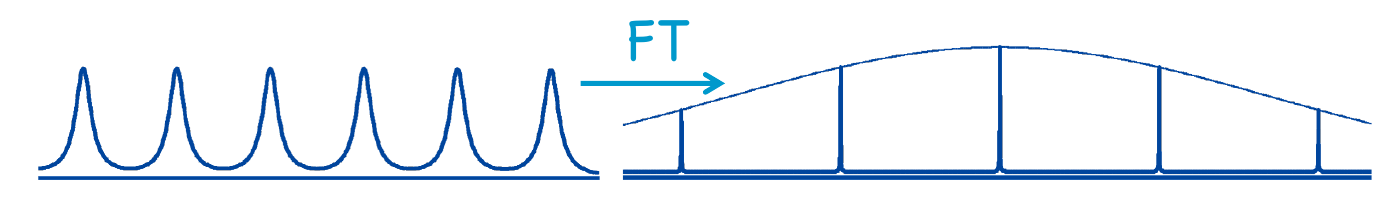
\includegraphics[width=0.5\textwidth]{figures/delta-smussate.png}
	\caption{Delta con inviluppo diverso dal caso periodico senza gas di elettroni.}
	\label{fig:fi}
\end{figure}
\noindent
Stringendo l'ampiezza dei picchi gaussiani si torna al caso precedente.
\subsection{Cristallo poliatomico.}
\label{subsec:Cristallo poliatomico.}
Per un cristallo poliatomico nella densità non abbiamo soltanto la somma sui vettori del reticolo, bensì anche sui vettori interni alla cella (che porteranno dei fattori di fase):
\[
	\rho (\v{r}) 
	=
	\sum_{I}^{} \sum_{i}^{} f_i(\v{r}-\v{r}_i - \v{R}_I)
	\xrightarrow[]{FT}
	\frac{N}{V} \sum_{J}^{} \sum_{i}^{} 
	\overline{f}_i(\v{k}) e^{i \v{k}\v{r}_i}\delta_{\v{k},\v{K}_J}
.\] 
Stiamo comunque assumendo di avere a che fare con un cristallo avente una orientazione specifica rispetto al vettore d'onda incidente: un monocristallo in cui i piani cristallini sono orientati tutti nella stessa direzione. Il risultato è una intensità della figura di diffrazione avente punti a diversa intensità, tali punti riflettono comunque la struttura interna del cristallo.\\
Se ho invece un policristallo (cristalli orientati a caso l'uno rispetto all'altro) allora possiamo mediare sull'angolo $\phi$ nel calcolo di $S(\v{q})$, in questo modo la figura di diffrazione saranno dei cerchi concentrici con intensità modulata. Tali cerchi soddisfano la condizione di Bragg:
\[
	2d\sin\theta=n\lambda
.\] 
\begin{figure}[H]
	\centering
	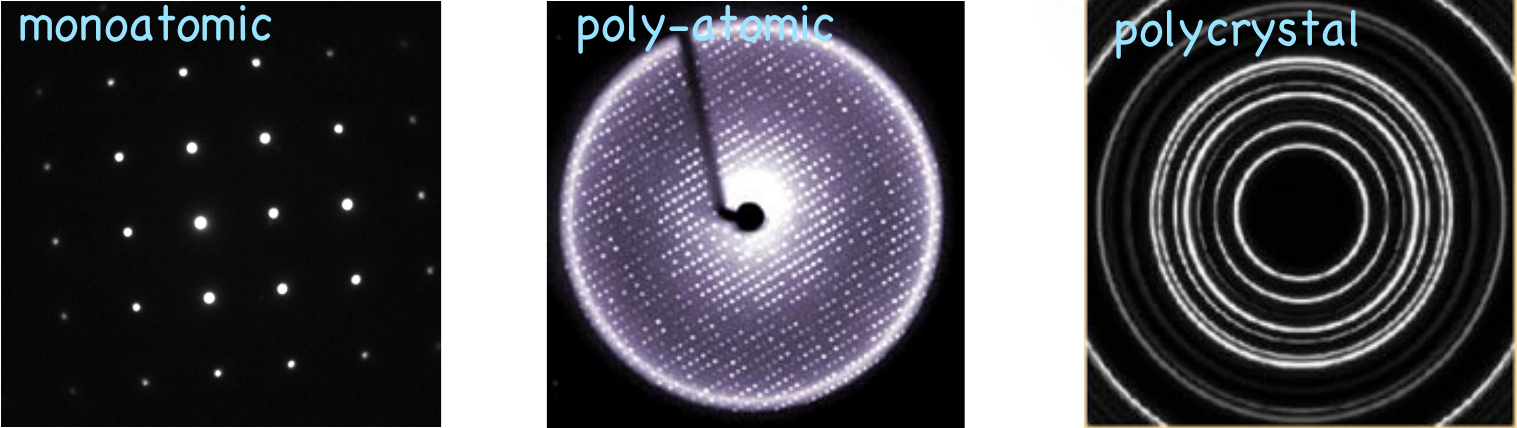
\includegraphics[width=0.6\textwidth]{figures/tipi-cristalli.png}
	\caption{Figura di diffrazione per varie tipologie di cristalli.}
	\label{fig:figures-tipi-cristalli-png}
\end{figure}
\subsection{Fattore di struttura statistica per gas perfetto}
\label{subsec:Fattore di struttura stati}
Nel caso di gas perfetto si ha che 
\begin{itemize}
	\item $\rho (\v{r})= \rho $ .
	\item $g(\v{r},\v{r'}) = 1$ (le particelle sono completamente scorrelate).
	\item $\overline{\rho }(\v{r},\v{r}') = \rho ^2$.
	\item $dN = 4\pi \rho r^2 dr$.
\end{itemize}
Di conseguenza abbiamo una $S(\v{q}) = 1$: una linea. Un gas non interagente da quindi uno scattering uniforme.
